% Options for packages loaded elsewhere
\PassOptionsToPackage{unicode}{hyperref}
\PassOptionsToPackage{hyphens}{url}
\PassOptionsToPackage{dvipsnames,svgnames*,x11names*}{xcolor}
%
\documentclass[
  ignorenonframetext,
]{beamer}
\usepackage{pgfpages}
\setbeamertemplate{caption}[numbered]
\setbeamertemplate{caption label separator}{: }
\setbeamercolor{caption name}{fg=normal text.fg}
\beamertemplatenavigationsymbolsempty
% Prevent slide breaks in the middle of a paragraph
\widowpenalties 1 10000
\raggedbottom
\setbeamertemplate{part page}{
  \centering
  \begin{beamercolorbox}[sep=16pt,center]{part title}
    \usebeamerfont{part title}\insertpart\par
  \end{beamercolorbox}
}
\setbeamertemplate{section page}{
  \centering
  \begin{beamercolorbox}[sep=12pt,center]{part title}
    \usebeamerfont{section title}\insertsection\par
  \end{beamercolorbox}
}
\setbeamertemplate{subsection page}{
  \centering
  \begin{beamercolorbox}[sep=8pt,center]{part title}
    \usebeamerfont{subsection title}\insertsubsection\par
  \end{beamercolorbox}
}
\AtBeginPart{
  \frame{\partpage}
}
\AtBeginSection{
  \ifbibliography
  \else
    \frame{\sectionpage}
  \fi
}
\AtBeginSubsection{
  \frame{\subsectionpage}
}
\usepackage{lmodern}
\usepackage{amssymb,amsmath}
\usepackage{ifxetex,ifluatex}
\ifnum 0\ifxetex 1\fi\ifluatex 1\fi=0 % if pdftex
  \usepackage[T1]{fontenc}
  \usepackage[utf8]{inputenc}
  \usepackage{textcomp} % provide euro and other symbols
\else % if luatex or xetex
  \usepackage{unicode-math}
  \defaultfontfeatures{Scale=MatchLowercase}
  \defaultfontfeatures[\rmfamily]{Ligatures=TeX,Scale=1}
\fi
\usetheme[]{AnnArbor}
\usecolortheme{dove}
% Use upquote if available, for straight quotes in verbatim environments
\IfFileExists{upquote.sty}{\usepackage{upquote}}{}
\IfFileExists{microtype.sty}{% use microtype if available
  \usepackage[]{microtype}
  \UseMicrotypeSet[protrusion]{basicmath} % disable protrusion for tt fonts
}{}
\makeatletter
\@ifundefined{KOMAClassName}{% if non-KOMA class
  \IfFileExists{parskip.sty}{%
    \usepackage{parskip}
  }{% else
    \setlength{\parindent}{0pt}
    \setlength{\parskip}{6pt plus 2pt minus 1pt}}
}{% if KOMA class
  \KOMAoptions{parskip=half}}
\makeatother
\usepackage{xcolor}
\IfFileExists{xurl.sty}{\usepackage{xurl}}{} % add URL line breaks if available
\IfFileExists{bookmark.sty}{\usepackage{bookmark}}{\usepackage{hyperref}}
\hypersetup{
  pdftitle={Statistical Inference: normal quantile plot},
  colorlinks=true,
  linkcolor=Maroon,
  filecolor=Maroon,
  citecolor=Blue,
  urlcolor=blue,
  pdfcreator={LaTeX via pandoc}}
\urlstyle{same} % disable monospaced font for URLs
\newif\ifbibliography
\usepackage{color}
\usepackage{fancyvrb}
\newcommand{\VerbBar}{|}
\newcommand{\VERB}{\Verb[commandchars=\\\{\}]}
\DefineVerbatimEnvironment{Highlighting}{Verbatim}{commandchars=\\\{\}}
% Add ',fontsize=\small' for more characters per line
\usepackage{framed}
\definecolor{shadecolor}{RGB}{248,248,248}
\newenvironment{Shaded}{\begin{snugshade}}{\end{snugshade}}
\newcommand{\AlertTok}[1]{\textcolor[rgb]{0.94,0.16,0.16}{#1}}
\newcommand{\AnnotationTok}[1]{\textcolor[rgb]{0.56,0.35,0.01}{\textbf{\textit{#1}}}}
\newcommand{\AttributeTok}[1]{\textcolor[rgb]{0.77,0.63,0.00}{#1}}
\newcommand{\BaseNTok}[1]{\textcolor[rgb]{0.00,0.00,0.81}{#1}}
\newcommand{\BuiltInTok}[1]{#1}
\newcommand{\CharTok}[1]{\textcolor[rgb]{0.31,0.60,0.02}{#1}}
\newcommand{\CommentTok}[1]{\textcolor[rgb]{0.56,0.35,0.01}{\textit{#1}}}
\newcommand{\CommentVarTok}[1]{\textcolor[rgb]{0.56,0.35,0.01}{\textbf{\textit{#1}}}}
\newcommand{\ConstantTok}[1]{\textcolor[rgb]{0.00,0.00,0.00}{#1}}
\newcommand{\ControlFlowTok}[1]{\textcolor[rgb]{0.13,0.29,0.53}{\textbf{#1}}}
\newcommand{\DataTypeTok}[1]{\textcolor[rgb]{0.13,0.29,0.53}{#1}}
\newcommand{\DecValTok}[1]{\textcolor[rgb]{0.00,0.00,0.81}{#1}}
\newcommand{\DocumentationTok}[1]{\textcolor[rgb]{0.56,0.35,0.01}{\textbf{\textit{#1}}}}
\newcommand{\ErrorTok}[1]{\textcolor[rgb]{0.64,0.00,0.00}{\textbf{#1}}}
\newcommand{\ExtensionTok}[1]{#1}
\newcommand{\FloatTok}[1]{\textcolor[rgb]{0.00,0.00,0.81}{#1}}
\newcommand{\FunctionTok}[1]{\textcolor[rgb]{0.00,0.00,0.00}{#1}}
\newcommand{\ImportTok}[1]{#1}
\newcommand{\InformationTok}[1]{\textcolor[rgb]{0.56,0.35,0.01}{\textbf{\textit{#1}}}}
\newcommand{\KeywordTok}[1]{\textcolor[rgb]{0.13,0.29,0.53}{\textbf{#1}}}
\newcommand{\NormalTok}[1]{#1}
\newcommand{\OperatorTok}[1]{\textcolor[rgb]{0.81,0.36,0.00}{\textbf{#1}}}
\newcommand{\OtherTok}[1]{\textcolor[rgb]{0.56,0.35,0.01}{#1}}
\newcommand{\PreprocessorTok}[1]{\textcolor[rgb]{0.56,0.35,0.01}{\textit{#1}}}
\newcommand{\RegionMarkerTok}[1]{#1}
\newcommand{\SpecialCharTok}[1]{\textcolor[rgb]{0.00,0.00,0.00}{#1}}
\newcommand{\SpecialStringTok}[1]{\textcolor[rgb]{0.31,0.60,0.02}{#1}}
\newcommand{\StringTok}[1]{\textcolor[rgb]{0.31,0.60,0.02}{#1}}
\newcommand{\VariableTok}[1]{\textcolor[rgb]{0.00,0.00,0.00}{#1}}
\newcommand{\VerbatimStringTok}[1]{\textcolor[rgb]{0.31,0.60,0.02}{#1}}
\newcommand{\WarningTok}[1]{\textcolor[rgb]{0.56,0.35,0.01}{\textbf{\textit{#1}}}}
\usepackage{longtable,booktabs}
\usepackage{caption}
% Make caption package work with longtable
\makeatletter
\def\fnum@table{\tablename~\thetable}
\makeatother
\usepackage{graphicx}
\makeatletter
\def\maxwidth{\ifdim\Gin@nat@width>\linewidth\linewidth\else\Gin@nat@width\fi}
\def\maxheight{\ifdim\Gin@nat@height>\textheight\textheight\else\Gin@nat@height\fi}
\makeatother
% Scale images if necessary, so that they will not overflow the page
% margins by default, and it is still possible to overwrite the defaults
% using explicit options in \includegraphics[width, height, ...]{}
\setkeys{Gin}{width=\maxwidth,height=\maxheight,keepaspectratio}
% Set default figure placement to htbp
\makeatletter
\def\fps@figure{htbp}
\makeatother
\setlength{\emergencystretch}{3em} % prevent overfull lines
\providecommand{\tightlist}{%
  \setlength{\itemsep}{0pt}\setlength{\parskip}{0pt}}
\setcounter{secnumdepth}{-\maxdimen} % remove section numbering
\usepackage{multicol}

\title{Statistical Inference: normal quantile plot}
\author{}
\date{\vspace{-2.5em}}

\begin{document}
\frame{\titlepage}

\begin{frame}[fragile]
knitr::opts\_chunk\(set(fig.height = 5) # knitr::opts_chunk\)set(echo =
FALSE) options(width=52) knitr::opts\_chunk\$set(dev = `pdf')

\begin{verbatim}






## The normal quantile plot

- see that normal distributions of data (or being normal enough) important
- only tools we have to assess this are histograms and maybe boxplots
- a better tool is **normal quantile plot**:
  - plot data against what you expect if data actually normal
  - look for points to follow a straight line, at least approx
- `ggplot` code: `aes` `sample`; geoms `stat_qq` and `stat_qq_line` 
  
## Kids learning to read





```r
ggplot(kids, aes(x = group, y = score)) + geom_boxplot()
\end{verbatim}

\includegraphics{inference_4a_R_slides_files/figure-beamer/unnamed-chunk-5-1.pdf}
Each group looks normal, or at least symmetric.
\end{frame}

\begin{frame}[fragile]{Get the groups separately}
\protect\hypertarget{get-the-groups-separately}{}
\begin{Shaded}
\begin{Highlighting}[]
\NormalTok{kids }\OperatorTok{\%\textgreater{}\%}\StringTok{ }\KeywordTok{filter}\NormalTok{(group }\OperatorTok{==}\StringTok{ "t"}\NormalTok{) {-}\textgreater{}}\StringTok{ }\NormalTok{treatment}
\NormalTok{kids }\OperatorTok{\%\textgreater{}\%}\StringTok{ }\KeywordTok{filter}\NormalTok{(group }\OperatorTok{==}\StringTok{ "c"}\NormalTok{) {-}\textgreater{}}\StringTok{ }\NormalTok{control}
\end{Highlighting}
\end{Shaded}

to check

\begin{Shaded}
\begin{Highlighting}[]
\NormalTok{treatment }\OperatorTok{\%\textgreater{}\%}\StringTok{ }\KeywordTok{count}\NormalTok{(group)}
\end{Highlighting}
\end{Shaded}

\begin{longtable}[]{@{}lr@{}}
\toprule
group & n\tabularnewline
\midrule
\endhead
t & 21\tabularnewline
\bottomrule
\end{longtable}

\begin{Shaded}
\begin{Highlighting}[]
\NormalTok{control }\OperatorTok{\%\textgreater{}\%}\StringTok{ }\KeywordTok{count}\NormalTok{(group)}
\end{Highlighting}
\end{Shaded}

\begin{longtable}[]{@{}lr@{}}
\toprule
group & n\tabularnewline
\midrule
\endhead
c & 23\tabularnewline
\bottomrule
\end{longtable}
\end{frame}

\begin{frame}[fragile]{The treatment group}
\protect\hypertarget{the-treatment-group}{}
\begin{Shaded}
\begin{Highlighting}[]
\KeywordTok{ggplot}\NormalTok{(treatment, }\KeywordTok{aes}\NormalTok{(}\DataTypeTok{sample =}\NormalTok{ score)) }\OperatorTok{+}\StringTok{ }
\StringTok{  }\KeywordTok{stat\_qq}\NormalTok{() }\OperatorTok{+}\StringTok{ }\KeywordTok{stat\_qq\_line}\NormalTok{()}
\end{Highlighting}
\end{Shaded}

\includegraphics{inference_4a_R_slides_files/figure-beamer/unnamed-chunk-8-1.pdf}
only problem here is lowest value a little too low (mild outlier).
\end{frame}

\begin{frame}[fragile]{Control group}
\protect\hypertarget{control-group}{}
\begin{Shaded}
\begin{Highlighting}[]
\KeywordTok{ggplot}\NormalTok{(control, }\KeywordTok{aes}\NormalTok{(}\DataTypeTok{sample =}\NormalTok{ score)) }\OperatorTok{+}\StringTok{ }
\StringTok{  }\KeywordTok{stat\_qq}\NormalTok{() }\OperatorTok{+}\StringTok{ }\KeywordTok{stat\_qq\_line}\NormalTok{()}
\end{Highlighting}
\end{Shaded}

\includegraphics{inference_4a_R_slides_files/figure-beamer/unnamed-chunk-9-1.pdf}

This time, highest value a little too high, but again, no real problem
with normality.
\end{frame}

\begin{frame}[fragile]{Facetting more than one sample}
\protect\hypertarget{facetting-more-than-one-sample}{}
Use the whole data set and facet by groups

\begin{Shaded}
\begin{Highlighting}[]
\KeywordTok{ggplot}\NormalTok{(kids, }\KeywordTok{aes}\NormalTok{(}\DataTypeTok{sample =}\NormalTok{ score)) }\OperatorTok{+}\StringTok{ }
\StringTok{  }\KeywordTok{stat\_qq}\NormalTok{() }\OperatorTok{+}\StringTok{ }\KeywordTok{stat\_qq\_line}\NormalTok{() }\OperatorTok{+}\StringTok{ }\KeywordTok{facet\_wrap}\NormalTok{(}\OperatorTok{\textasciitilde{}}\NormalTok{group)}
\end{Highlighting}
\end{Shaded}

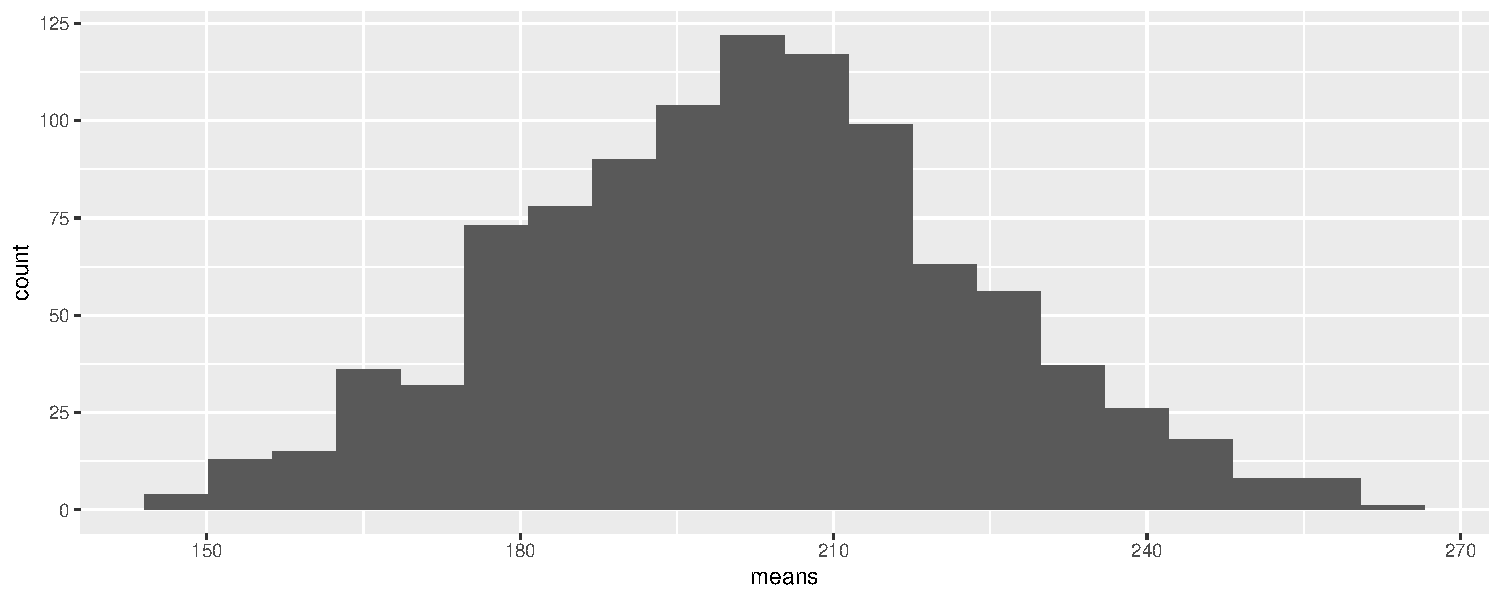
\includegraphics{inference_4a_R_slides_files/figure-beamer/unnamed-chunk-10-1.pdf}
\end{frame}

\begin{frame}[fragile]{Blue Jays attendances, skewed to right}
\protect\hypertarget{blue-jays-attendances-skewed-to-right}{}
\begin{Shaded}
\begin{Highlighting}[]
\KeywordTok{ggplot}\NormalTok{(jays, }\KeywordTok{aes}\NormalTok{(}\DataTypeTok{x =}\NormalTok{ attendance)) }\OperatorTok{+}\StringTok{ }\KeywordTok{geom\_histogram}\NormalTok{(}\DataTypeTok{bins =} \DecValTok{6}\NormalTok{)}
\end{Highlighting}
\end{Shaded}

\includegraphics{inference_4a_R_slides_files/figure-beamer/unnamed-chunk-12-1.pdf}
\end{frame}

\begin{frame}[fragile]{On a normal quantile plot}
\protect\hypertarget{on-a-normal-quantile-plot}{}
\begin{Shaded}
\begin{Highlighting}[]
\KeywordTok{ggplot}\NormalTok{(jays, }\KeywordTok{aes}\NormalTok{(}\DataTypeTok{sample =}\NormalTok{ attendance)) }\OperatorTok{+}\StringTok{ }
\StringTok{  }\KeywordTok{stat\_qq}\NormalTok{() }\OperatorTok{+}\StringTok{ }\KeywordTok{stat\_qq\_line}\NormalTok{()}
\end{Highlighting}
\end{Shaded}

\includegraphics{inference_4a_R_slides_files/figure-beamer/unnamed-chunk-13-1.pdf}

\begin{itemize}
\tightlist
\item
  Attendances at low end too bunched up: skewed to right.
\item
  Right-skewness can also show up as highest values being too high, or
  as a curved pattern in the points.
\end{itemize}
\end{frame}

\begin{frame}{More normal quantile plots}
\protect\hypertarget{more-normal-quantile-plots}{}
\begin{itemize}
\tightlist
\item
  How straight does a normal quantile plot have to be?
\item
  There is randomness in real data, so even a normal quantile plot from
  normal data won't look perfectly straight.
\item
  With a small sample, can look not very straight even from normal data.
\item
  Looking for systematic departure from a straight line; random wiggles
  ought not to concern us.
\item
  Look at some examples where we know the answer, so that we can see
  what to expect.
\end{itemize}
\end{frame}

\begin{frame}[fragile]{Normal data, large sample}
\protect\hypertarget{normal-data-large-sample}{}
\begin{Shaded}
\begin{Highlighting}[]
\NormalTok{d=}\KeywordTok{tibble}\NormalTok{(}\DataTypeTok{x=}\KeywordTok{rnorm}\NormalTok{(}\DecValTok{200}\NormalTok{))}
\KeywordTok{ggplot}\NormalTok{(d,}\KeywordTok{aes}\NormalTok{(}\DataTypeTok{x=}\NormalTok{x))}\OperatorTok{+}\KeywordTok{geom\_histogram}\NormalTok{(}\DataTypeTok{bins=}\DecValTok{10}\NormalTok{)}
\end{Highlighting}
\end{Shaded}

\includegraphics{inference_4a_R_slides_files/figure-beamer/unnamed-chunk-14-1.pdf}
\end{frame}

\begin{frame}[fragile]{The normal quantile plot}
\protect\hypertarget{the-normal-quantile-plot}{}
\begin{Shaded}
\begin{Highlighting}[]
\KeywordTok{ggplot}\NormalTok{(d,}\KeywordTok{aes}\NormalTok{(}\DataTypeTok{sample=}\NormalTok{x))}\OperatorTok{+}\KeywordTok{stat\_qq}\NormalTok{()}\OperatorTok{+}\KeywordTok{stat\_qq\_line}\NormalTok{()}
\end{Highlighting}
\end{Shaded}

\includegraphics{inference_4a_R_slides_files/figure-beamer/unnamed-chunk-15-1.pdf}
\end{frame}

\begin{frame}[fragile]{Normal data, small sample}
\protect\hypertarget{normal-data-small-sample}{}
\begin{itemize}
\tightlist
\item
  Not so convincingly normal, but not obviously skewed:
\end{itemize}

\begin{Shaded}
\begin{Highlighting}[]
\NormalTok{d=}\KeywordTok{tibble}\NormalTok{(}\DataTypeTok{x=}\KeywordTok{rnorm}\NormalTok{(}\DecValTok{20}\NormalTok{))}
\KeywordTok{ggplot}\NormalTok{(d,}\KeywordTok{aes}\NormalTok{(}\DataTypeTok{x=}\NormalTok{x))}\OperatorTok{+}\KeywordTok{geom\_histogram}\NormalTok{(}\DataTypeTok{bins=}\DecValTok{5}\NormalTok{)}
\end{Highlighting}
\end{Shaded}

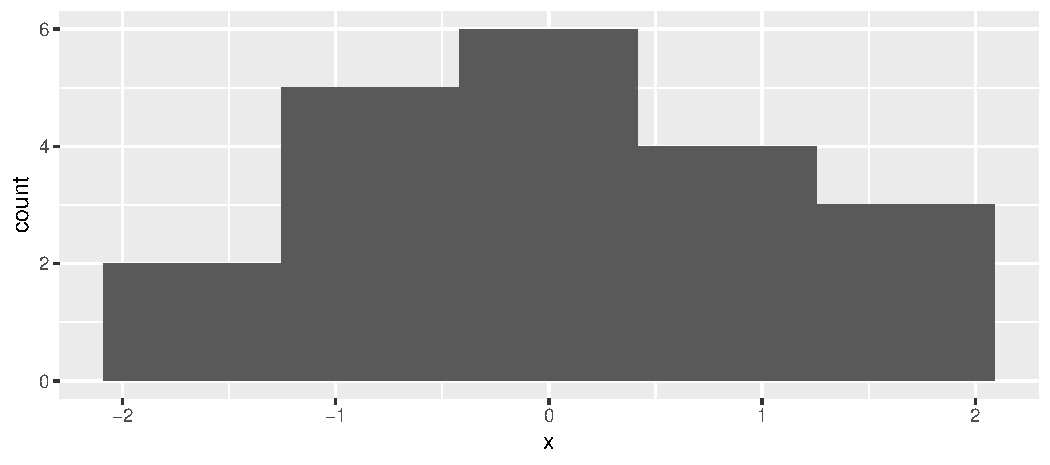
\includegraphics{inference_4a_R_slides_files/figure-beamer/normal-small-1.pdf}
\end{frame}

\begin{frame}[fragile]{The normal quantile plot}
\protect\hypertarget{the-normal-quantile-plot-1}{}
Good, apart from the highest and lowest points being slightly off. I'd
call this good:

\begin{Shaded}
\begin{Highlighting}[]
\KeywordTok{ggplot}\NormalTok{(d,}\KeywordTok{aes}\NormalTok{(}\DataTypeTok{sample=}\NormalTok{x))}\OperatorTok{+}\KeywordTok{stat\_qq}\NormalTok{()}\OperatorTok{+}\KeywordTok{stat\_qq\_line}\NormalTok{()}
\end{Highlighting}
\end{Shaded}

\includegraphics{inference_4a_R_slides_files/figure-beamer/unnamed-chunk-17-1.pdf}
\end{frame}

\begin{frame}[fragile]{Chi-squared data, \emph{df} = 10}
\protect\hypertarget{chi-squared-data-df-10}{}
Somewhat skewed to right:

\begin{Shaded}
\begin{Highlighting}[]
\NormalTok{d=}\KeywordTok{tibble}\NormalTok{(}\DataTypeTok{x=}\KeywordTok{rchisq}\NormalTok{(}\DecValTok{100}\NormalTok{,}\DecValTok{10}\NormalTok{))}
\KeywordTok{ggplot}\NormalTok{(d,}\KeywordTok{aes}\NormalTok{(}\DataTypeTok{x=}\NormalTok{x))}\OperatorTok{+}\KeywordTok{geom\_histogram}\NormalTok{(}\DataTypeTok{bins=}\DecValTok{10}\NormalTok{)}
\end{Highlighting}
\end{Shaded}

\includegraphics{inference_4a_R_slides_files/figure-beamer/unnamed-chunk-18-1.pdf}
\end{frame}

\begin{frame}[fragile]{The normal quantile plot}
\protect\hypertarget{the-normal-quantile-plot-2}{}
Somewhat opening-up curve:

\begin{Shaded}
\begin{Highlighting}[]
\KeywordTok{ggplot}\NormalTok{(d,}\KeywordTok{aes}\NormalTok{(}\DataTypeTok{sample=}\NormalTok{x))}\OperatorTok{+}\KeywordTok{stat\_qq}\NormalTok{()}\OperatorTok{+}\KeywordTok{stat\_qq\_line}\NormalTok{()}
\end{Highlighting}
\end{Shaded}

\includegraphics{inference_4a_R_slides_files/figure-beamer/unnamed-chunk-19-1.pdf}
\end{frame}

\begin{frame}[fragile]{Chi-squared data, df = 3}
\protect\hypertarget{chi-squared-data-df-3}{}
Definitely skewed to right:

\begin{Shaded}
\begin{Highlighting}[]
\NormalTok{d=}\KeywordTok{tibble}\NormalTok{(}\DataTypeTok{x=}\KeywordTok{rchisq}\NormalTok{(}\DecValTok{100}\NormalTok{,}\DecValTok{3}\NormalTok{))}
\KeywordTok{ggplot}\NormalTok{(d,}\KeywordTok{aes}\NormalTok{(}\DataTypeTok{x=}\NormalTok{x))}\OperatorTok{+}\KeywordTok{geom\_histogram}\NormalTok{(}\DataTypeTok{bins=}\DecValTok{10}\NormalTok{)}
\end{Highlighting}
\end{Shaded}

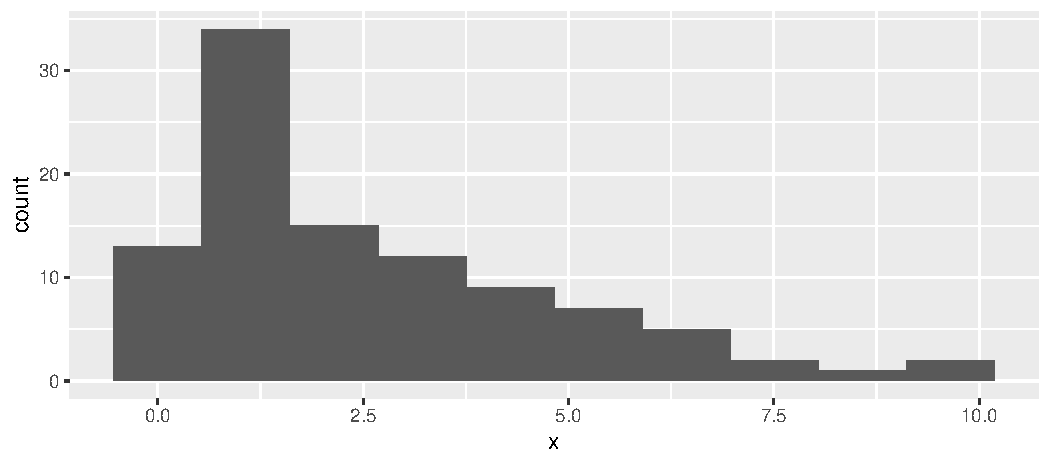
\includegraphics{inference_4a_R_slides_files/figure-beamer/chisq-small-df-1.pdf}
\end{frame}

\begin{frame}[fragile]{The normal quantile plot}
\protect\hypertarget{the-normal-quantile-plot-3}{}
Clear upward-opening curve:

\begin{Shaded}
\begin{Highlighting}[]
\KeywordTok{ggplot}\NormalTok{(d,}\KeywordTok{aes}\NormalTok{(}\DataTypeTok{sample=}\NormalTok{x))}\OperatorTok{+}\KeywordTok{stat\_qq}\NormalTok{()}\OperatorTok{+}\KeywordTok{stat\_qq\_line}\NormalTok{()}
\end{Highlighting}
\end{Shaded}

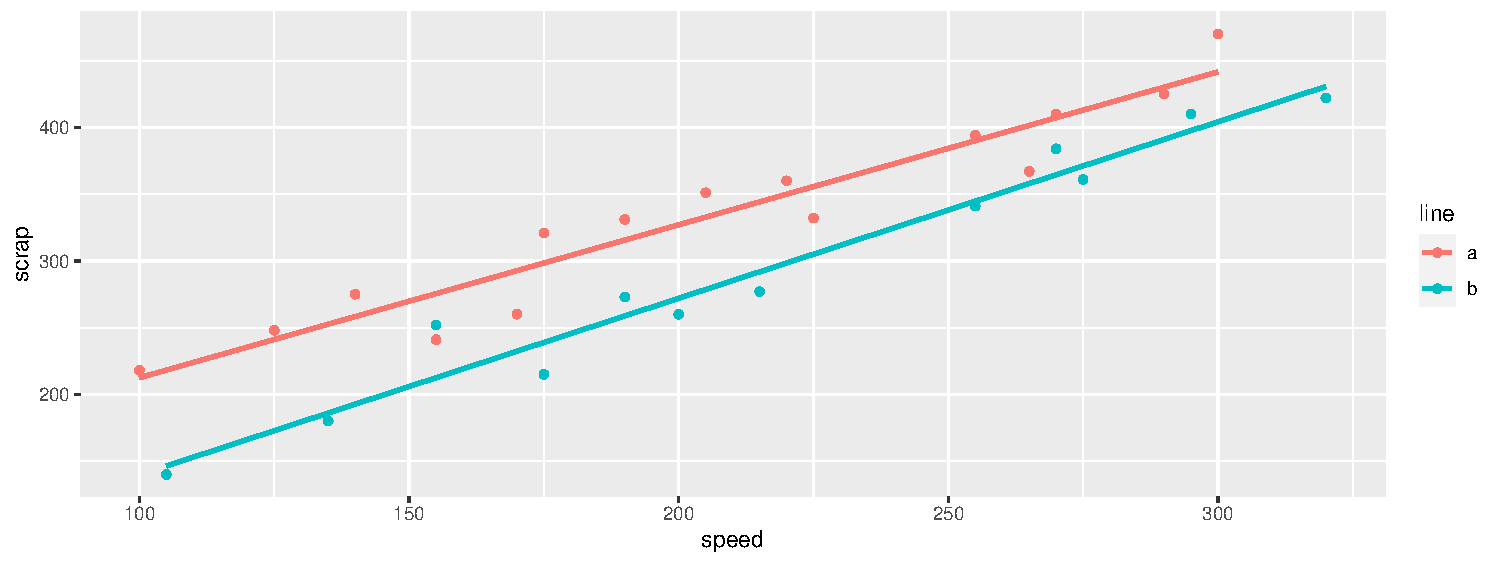
\includegraphics{inference_4a_R_slides_files/figure-beamer/unnamed-chunk-20-1.pdf}
\end{frame}

\begin{frame}[fragile]{t-distributed data, df = 3}
\protect\hypertarget{t-distributed-data-df-3}{}
Long tails (or a very sharp peak):

\begin{Shaded}
\begin{Highlighting}[]
\NormalTok{d=}\KeywordTok{tibble}\NormalTok{(}\DataTypeTok{x=}\KeywordTok{rt}\NormalTok{(}\DecValTok{300}\NormalTok{,}\DecValTok{3}\NormalTok{))}
\KeywordTok{ggplot}\NormalTok{(d,}\KeywordTok{aes}\NormalTok{(}\DataTypeTok{x=}\NormalTok{x))}\OperatorTok{+}\KeywordTok{geom\_histogram}\NormalTok{(}\DataTypeTok{bins=}\DecValTok{10}\NormalTok{)}
\end{Highlighting}
\end{Shaded}

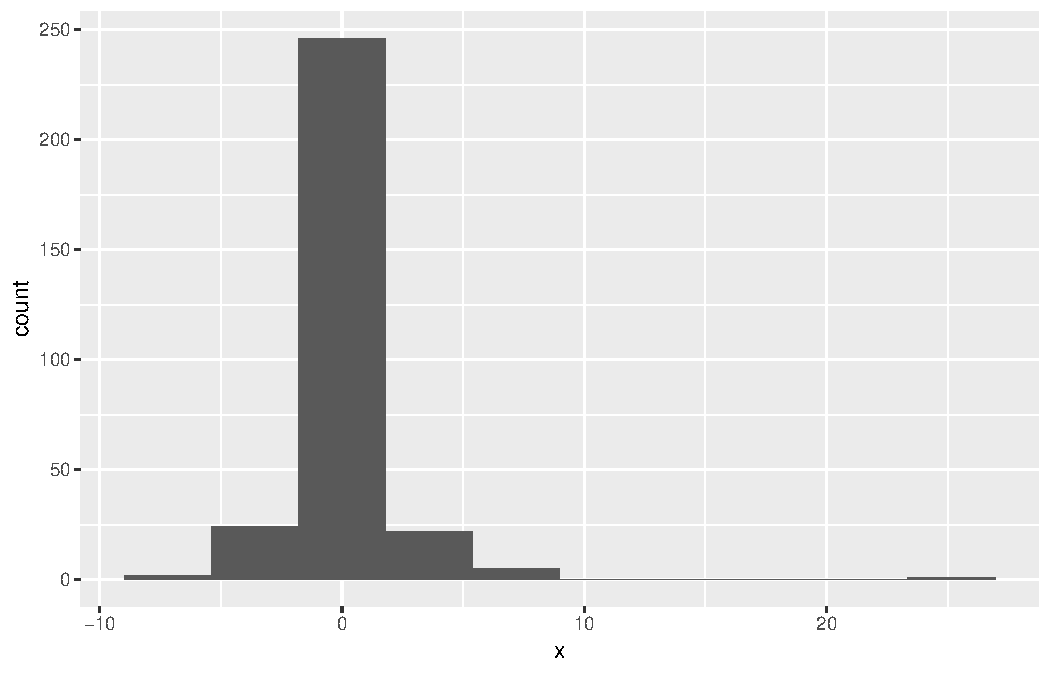
\includegraphics{inference_4a_R_slides_files/figure-beamer/t-small-1.pdf}
\end{frame}

\begin{frame}[fragile]{The normal quantile plot}
\protect\hypertarget{the-normal-quantile-plot-4}{}
Low values too low and high values too high for normal.

\begin{Shaded}
\begin{Highlighting}[]
\KeywordTok{ggplot}\NormalTok{(d,}\KeywordTok{aes}\NormalTok{(}\DataTypeTok{sample=}\NormalTok{x))}\OperatorTok{+}\KeywordTok{stat\_qq}\NormalTok{()}\OperatorTok{+}\KeywordTok{stat\_qq\_line}\NormalTok{()}
\end{Highlighting}
\end{Shaded}

\includegraphics{inference_4a_R_slides_files/figure-beamer/unnamed-chunk-21-1.pdf}
\end{frame}

\begin{frame}{Summary}
\protect\hypertarget{summary}{}
On a normal quantile plot:

\begin{itemize}
\tightlist
\item
  points following line (with some small wiggles): normal.
\item
  kind of deviation from a straight line indicates kind of nonnormality:

  \begin{itemize}
  \tightlist
  \item
    a few highest point(s) too high and/or lowest too low: outliers
  \item
    else see how points at each end off the line:
  \end{itemize}

  \begin{tabular}{lcc}
  & \multicolumn{2}{c}{High points}\\
  Low points & Too low & too high\\
  \hline
  Too low & Skewed left & Long tails\\
  Too high & Short tails & Skewed right \\
  \hline

  \end{tabular}
\item
  short-tailed distribution OK for \(t\) (mean still good), but others
  problematic (depending on sample size).
\end{itemize}
\end{frame}

\end{document}
